\section{Hasil dan Pembahasan}
\label{sec:hasildanpembahasan}

Dilakukan pengujian dan analisis terhadap perancangan dan implementasi yang telah di desain sebelumnya. Pengujian yang dilakukan meliputi pengujian Sensor Load Cell terhadap Robot dan Sistem Keseimbangan Robot. 

\begin{enumerate}[label=\Alph*.]

    \item Pengujian Karakterisasi Pada Masing-Masing Sensor Load Cell
    \label{subsec:hasil-pembahasan-karakterisasi}

        \hspace*{1em} Pengujian kalibrasi sensor load cell dilakukan dengan menggunakan lima bandul referensi massa (50g, 100g, 200g, 500g, dan 1000g) untuk menentukan koefisien gradien dan konstanta tare weight. Load cell dihubungkan dalam dua kelompok: Load Cell 1 dan 4, serta Load Cell 2 dan 3. 

        \begin{table}[h]
            \centering
            \caption{Hasil Karakterisasi Load Cell Pertama}
            \begin{tabular}{|c|c|c|}
                \hline
                \textbf{Berat Aktual (gr)} & \textbf{Load Cell 1 Pembacaan (gr)} & \textbf{Error (gr)} \\
                \hline
                50    & 50    & 0   \\
                100   & 101   & 1   \\
                200   & 202   & 2   \\
                500   & 505   & 5   \\
                1000  & 1004  & 4   \\
                \hline
            \end{tabular}
            \label{tab:Kalibrasi_Load_Cell_1}
        \end{table}

        \begin{table}[h]
            \centering
            \caption{Hasil Karakterisasi Load Cell Kedua}
            \begin{tabular}{|c|c|c|}
                \hline
                \textbf{Berat Aktual (gr)} & \textbf{Load Cell 2 Pembacaan (gr)} & \textbf{Error (gr)} \\
                \hline
                50        & 50        & 0   \\
                100       & 100       & 0   \\
                200       & 200       & 0   \\
                500       & 500       & 0   \\
                1000      & 994       & 6   \\           
                \hline
        \end{tabular}
        \label{tab:Kalibrasi_Load_Cell_2}
        \end{table}

        \begin{table}[h]
            \centering
            \caption{Hasil Karakterisasi Load Cell Ketiga}
            \begin{tabular}{|c|c|c|}
                \hline
                \textbf{Berat Aktual (gr)} & \textbf{Load Cell 3 Pembacaan (gr)} & \textbf{Error (gr)} \\
                \hline
                50        & 50        & 0    \\    
                100       & 103       & 3    \\    
                200       & 203       & 3    \\    
                500       & 494       & 6    \\    
                1000      & 981       & 19   \\               
                \hline
        \end{tabular}
        \label{tab:Kalibrasi_Load_Cell_3}
        \end{table}

        \begin{table}[h]
            \centering
            \caption{Hasil Karakterisasi Load Cell Keempat}
            \begin{tabular}{|c|c|c|}
                \hline
                \textbf{Berat Aktual (gr)} & \textbf{Load Cell 4 Pembacaan (gr)} & \textbf{Error (gr)} \\
                \hline
                50        & 50        & 0   \\     
                100       & 97        & 3   \\     
                200       & 204       & 4   \\     
                500       & 500       & 0   \\     
                1000      & 1003      & 3   \\                
                \hline
        \end{tabular}
        \label{tab:Kalibrasi_Load_Cell_4}
        \end{table}
    
        
        \hspace*{1em} Data pembacaan digital dari load cell dihitung menjadi massa aktual menggunakan persamaan kalibrasi, dan kesalahan diukur dengan membandingkan hasil dengan massa aktual. Hasil pengukuran menunjukkan kesalahan bervariasi antara 0 hingga 20 gram. Meskipun tidak sepenuhnya linear, persamaan kalibrasi yang digunakan cukup akurat dengan toleransi kesalahan sebesar 5\%.

    \item Pengujian Tekanan Pada Telapak Kaki
    \label{subsec:hasil-pembahasan-tekanan}

        \hspace*{1em} Pengujian ini dilakukan untuk mendapatkan data tekanan yang dihasilkan oleh kaki kanan dan kaki kiri ketika diberikan beban secara merata. Data tekanan yang dihasilkan oleh kaki kanan dan kaki kiri dapat dilihat pada Tabel \ref{tab:pengukuran_berat_kaki_kiri} dan Tabel \ref{tab:pengukuran_berat_kaki_kanan}.

        \begin{table}[h!]
            \centering
            \caption{Tabel Pembacaan Tekanan untuk Kaki Kiri}
            \begin{tabular}{|c|c|c|}
                \hline
                \textbf{Berat Aktual (gr)} & \textbf{Pembacaan (gr)} & \textbf{Error (gr)} \\
                \hline
                50    & 52    & 2   \\
                100   & 110   & 10  \\
                200   & 220   & 20  \\
                300   & 304   & 4   \\
                500   & 512   & 12  \\
                700   & 701   & 1   \\
                1000  & 1050  & 50  \\
                1300  & 1325  & 25  \\
                1500  & 1512  & 12  \\
                1800  & 1788  & 12  \\
                \hline
                \textbf{Rata-rata Error (gr)} & \multicolumn{2}{c|}{\textbf{14.8}} \\
                \hline
            \end{tabular}
            \label{tab:pengukuran_berat_kaki_kiri}
        \end{table}

        \begin{table}[h!]
            \centering
            \caption{Tabel Pembacaan Tekanan untuk Kaki Kanan}
            \begin{tabular}{|c|c|c|}
                \hline
                \textbf{Berat Aktual (gr)} & \textbf{Pembacaan (gr)} & \textbf{Error (gr)} \\
                \hline
                50    & 46    & 4    \\
                100   & 98    & 2    \\
                200   & 215   & 15   \\
                300   & 325   & 25   \\
                500   & 505   & 5    \\
                700   & 722   & 22   \\
                1000  & 1025  & 25   \\
                1300  & 1347  & 47   \\
                1500  & 1500  & 0    \\
                1800  & 1819  & 19   \\
                \hline
                \textbf{Rata-rata Error (gr)} & \multicolumn{2}{c|}{\textbf{16.4}} \\
                \hline
            \end{tabular}
            \label{tab:pengukuran_berat_kaki_kanan}
        \end{table}

        \hspace*{1em} Berdasarkan hasil pengujian, rata-rata kesalahan yang dihasilkan oleh kaki kiri adalah 14.8 gram dan kaki kanan adalah 16.4 gram.

    \item Pengujian Pusat Tekanan Terhadap Robot
    \label{subsec:hasil-pembahasan-pusat-tekanan}

        \hspace*{1em} Pengujian ini dilakukan dengan menggerakkan robot dalam pola berjalan dan mengambil data input dari sensor tekanan dengan interval 50 ms. Tujuan pengujian ini adalah untuk mendapatkan data pusat tekanan saat robot melakukan gerakan berjalan, serta untuk mengamati bagaimana pusat tekanan berubah selama gerakan berlangsung. Hasil Pengujian Pusat Tekanan Terhadap Robot dapat dilihat pada Gambar \ref{fig:pusat_tekanan_robot}.

        \begin{figure}[h]
            \centering
            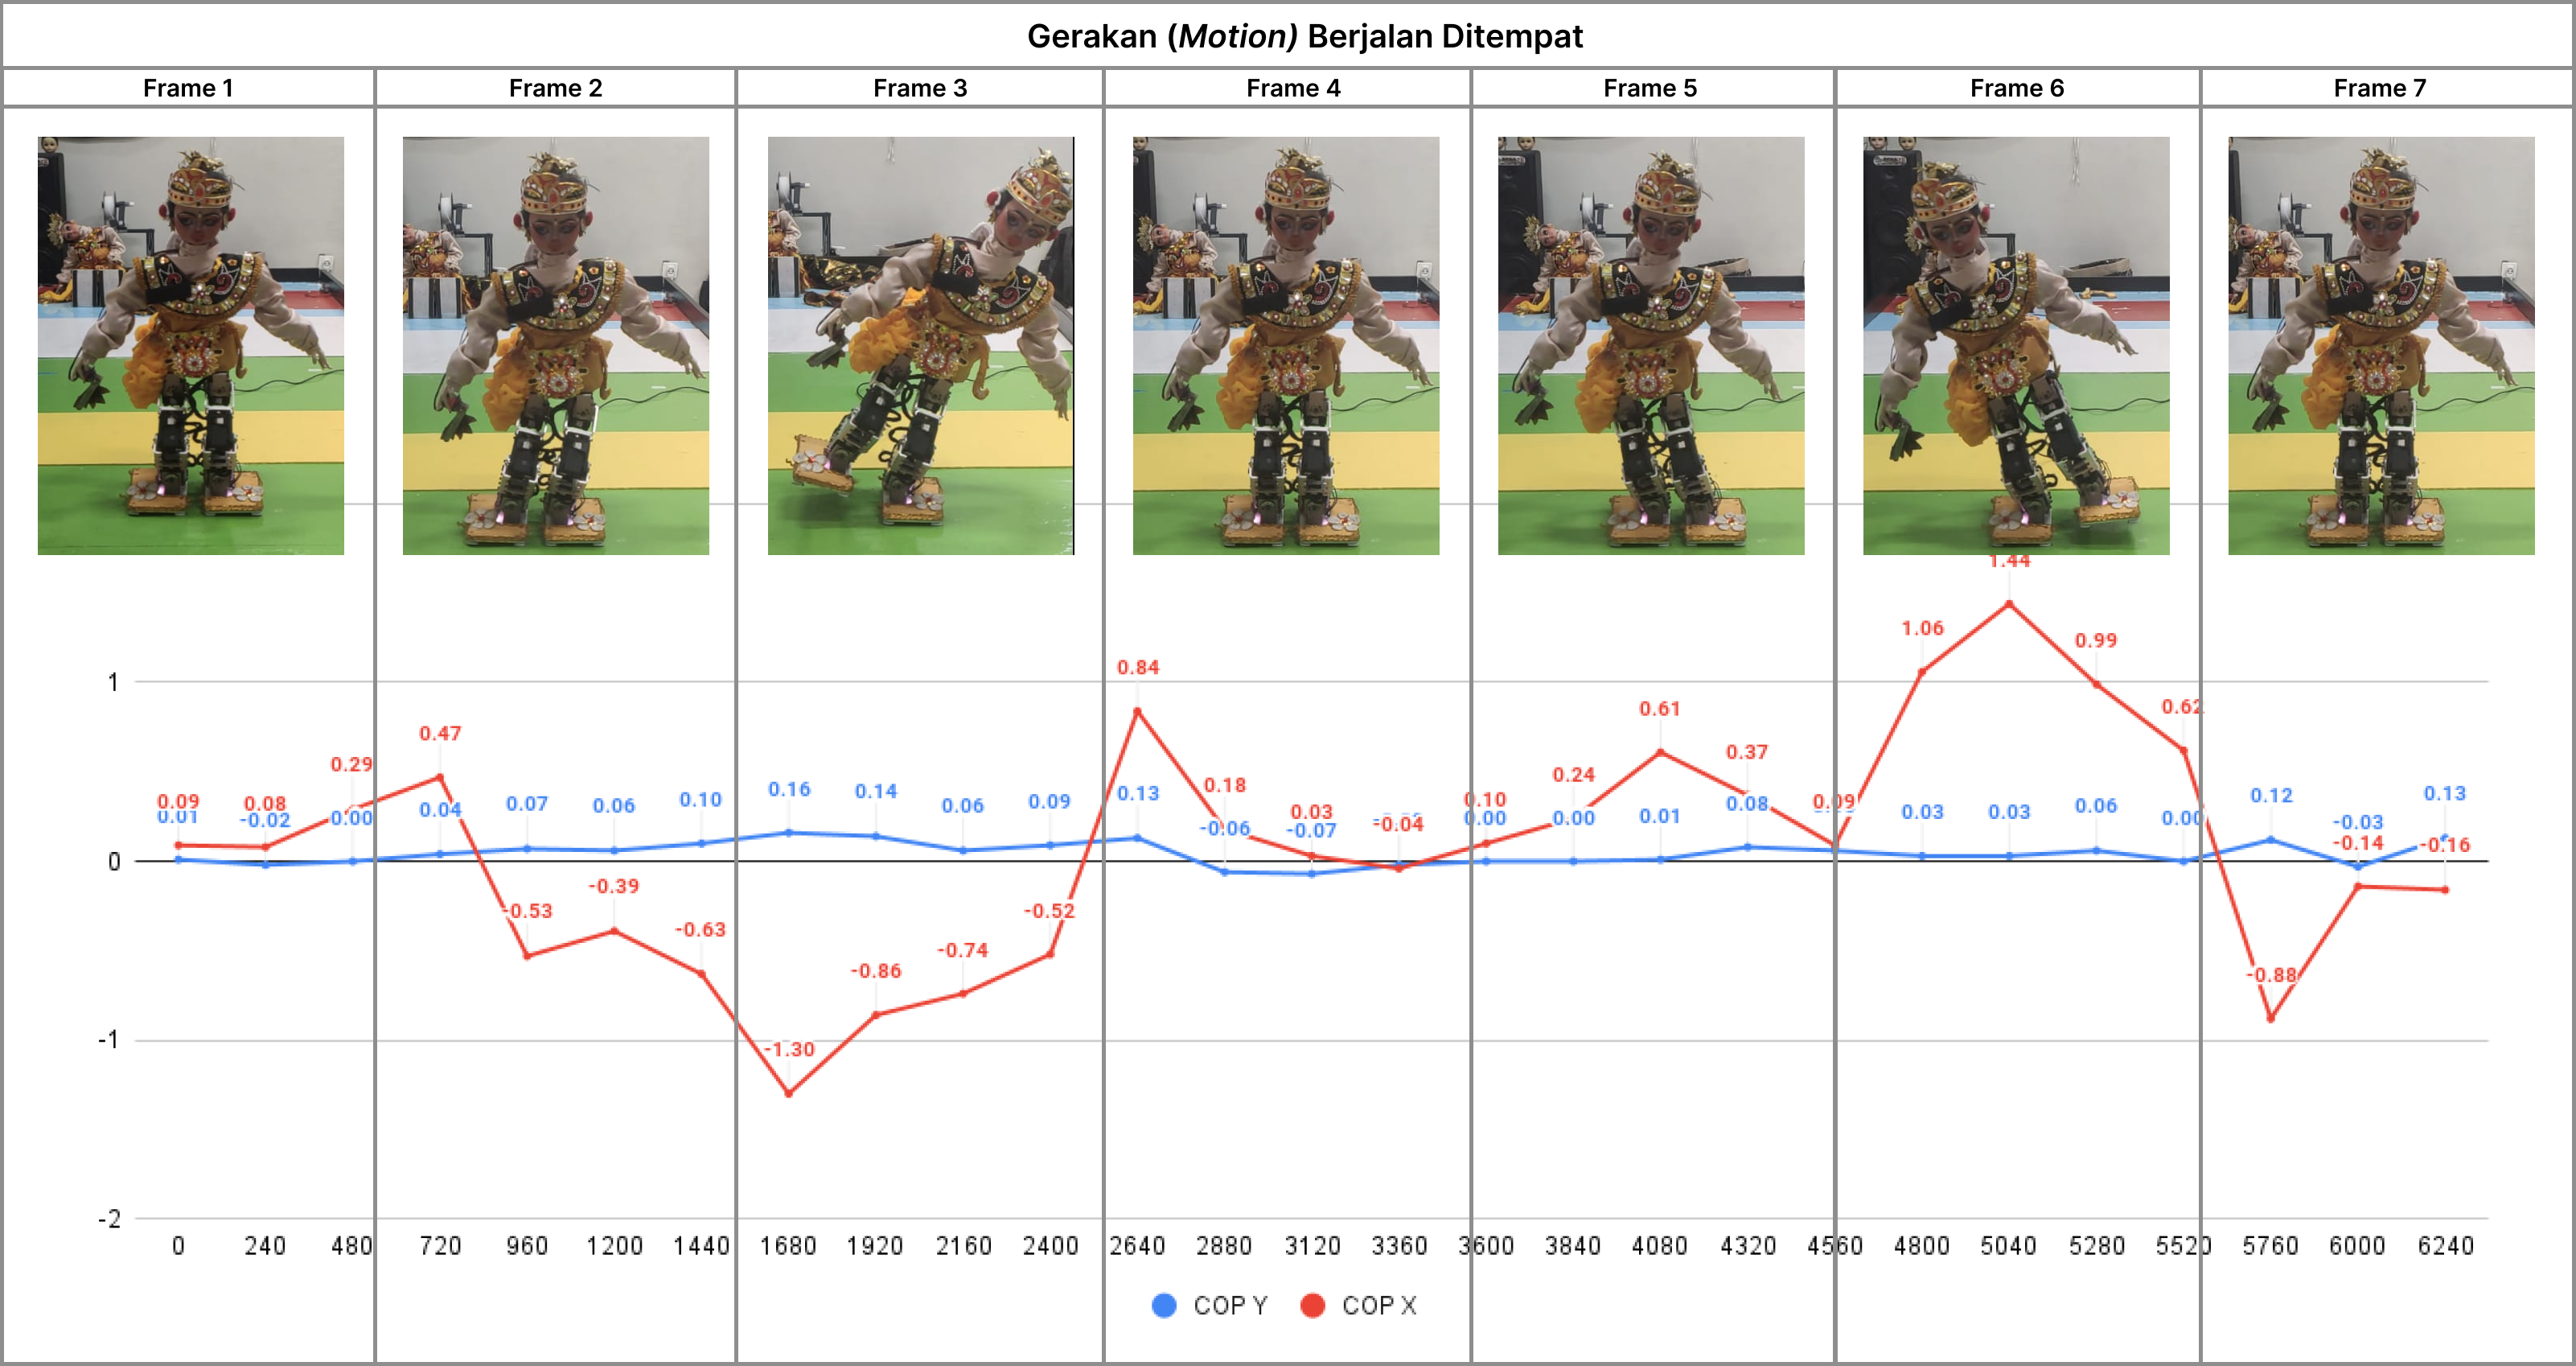
\includegraphics[width=0.45\textwidth]{gambar/motion_berjalan.png}
            \caption{Grafik Pusat Tekanan Ketika Robot Berjalan Di Tempat}
            \label{fig:pusat_tekanan_robot}
        \end{figure}

        \hspace*{1em} Hasil pengujian menunjukkan bahwa pusat tekanan berubah secara dinamis selama robot melakukan gerakan berjalan. Ketika robot mengangkat kaki kanan, pusat tekanan berpindah ke kaki kiri, dan nilai pusat tekan pada sumbu X memiliki nilai maksimum sebesar 1.44. Sebaliknya, ketika robot mengangkat kaki kiri, pusat tekanan berpindah ke kaki kanan, dan nilai pusat tekan pada sumbu X memiliki nilai minimum sebesar -1.3. Pada sumbu Y, nilai pusat tekanan berada pada rentang 0.16 hingga -0.06, yang menunjukkan bahwa pusat tekanan berada di tengah-tengah telapak kaki.

    \item Pengujian Sistem Kontrol PID
    \label{subsec:hasil-pembahasan-pid}

        \hspace*{1em} Pengujian ini, akan membandingkan pengaruh parameter \(K_p\) terhadap performa sistem kontrol PID. Pengujian dilakukan dengan mengukur Root Mean Square (RMS) dan hasil pengujian pada gerakan angkat kaki kanan dan kiri. 

        \begin{table}[h]
            \centering
            \caption{Root Mean Square (RMS) pada Pengujian Pengaruh Parameter P}
            \begin{tabular}{|c|c|}
            \hline
            \textbf{PID} & \textbf{RMS Error} \\
            \hline
            $K_p = 0.00$ & 0.7598 \\
            $K_p = 0.05$ & 0.7690 \\
            $K_p = 0.10$ & 0.7779 \\
            $K_p = 0.15$ & 0.8145 \\
            $K_p = 0.20$ & 0.8870 \\
            $K_p = 0.25$ & 0.8801 \\
            \hline
            \end{tabular}
            \label{tab:ems_p}
        \end{table}

        \begin{table}[h]
            \centering
            \caption{Hasil Pengujian Pengaruh Parameter P pada Kontroler PID, Gerakan Angkat Kaki Kanan}
            \begin{tabular}{|c|c|c|c|}
                \hline
                \textbf{PID} & \textbf{Fall} & \textbf{Not Fall} & \textbf{Success} \\
                \hline
                $K_p = 0.00$ & 6 & 0 & 0   \% \\
                $K_p = 0.05$ & 6 & 0 & 0   \% \\
                $K_p = 0.10$ & 0 & 6 & 100 \% \\
                $K_p = 0.15$ & 1 & 5 & 83  \% \\
                $K_p = 0.20$ & 0 & 6 & 100 \% \\
                $K_p = 0.25$ & 2 & 4 & 66  \% \\            
                \hline
            \end{tabular}
            \label{tab:pengujian_p_kanan}
        \end{table}

        \begin{table}[h]
            \centering
            \caption{Hasil Pengujian Pengaruh Parameter P pada Kontroler PID, Gerakan Angkat Kaki Kiri}
            \begin{tabular}{|c|c|c|c|}
                \hline
                \textbf{PID} & \textbf{Fall} & \textbf{Not Fall} & \textbf{Success} \\
                \hline
                $K_p = 0.00$ & 6 & 0 & 0   \% \\
                $K_p = 0.05$ & 6 & 0 & 0   \% \\
                $K_p = 0.10$ & 0 & 6 & 100  \% \\
                $K_p = 0.15$ & 1 & 5 & 83  \% \\
                $K_p = 0.20$ & 1 & 5 & 83  \% \\
                $K_p = 0.25$ & 0 & 6 & 100 \% \\            
                \hline
            \end{tabular}
            \label{tab:pengujian_p_kiri}
        \end{table}

        \hspace*{1em} Dari hasil pengujian yang disajikan dalam tabel-tabel tersebut, nilai optimal dari parameter \(K_p\) yang memungkinkan robot untuk menjaga keseimbangan dengan baik berkisar antara 0.10 hingga 0.20. Pada nilai \(K_p\) = 0.00 dan \(K_p\) = 0.05, semua pengujian gagal dengan robot selalu jatuh, menunjukkan bahwa kontrol PID tidak efektif pada nilai tersebut. Sebaliknya, nilai \(K_p = 0.10\) menunjukkan performa terbaik dengan keberhasilan 100\% dalam menjaga keseimbangan robot pada gerakan mengangkat kaki kanan maupun kaki kiri di kemiringan 3 derajat. 

        \hspace*{1em} Kemudian dari hasil \textit{Root Mean Square (RMS)} yang disajikan dalam Tabel \ref{tab:ems_p}, terlihat bahwa nilai RMS terkecil diperoleh pada \(K_p = 0.10\), menunjukkan ketidakakuratan terkecil dalam sistem pada nilai ini. 

\end{enumerate}